\documentclass[conference,letterpaper,10pt]{IEEEtran}
\IEEEoverridecommandlockouts

\usepackage[T1]{fontenc}
\usepackage[utf8]{inputenc}
\usepackage{cite}
\usepackage{amsmath,amssymb}
\usepackage{graphicx}
\usepackage{booktabs}
\usepackage{array}
\usepackage{tabularx}
\usepackage{url}
\graphicspath{{figures/}}



% Keep floats close to their first mention while preserving IEEE layout.
\renewcommand{\topfraction}{0.95}
\renewcommand{\dbltopfraction}{0.95}
\renewcommand{\textfraction}{0.05}
\renewcommand{\floatpagefraction}{0.85}
\renewcommand{\dblfloatpagefraction}{0.85}
\setcounter{topnumber}{4}
\setcounter{totalnumber}{6}
\setcounter{dbltopnumber}{3}
\setlength{\textfloatsep}{7pt plus 2pt minus 2pt}
\setlength{\floatsep}{7pt plus 2pt minus 2pt}
\setlength{\dbltextfloatsep}{7pt plus 2pt minus 2pt}
\newcolumntype{Y}{>{\raggedright\arraybackslash}X}
\newcommand{\method}[1]{\textsc{#1}}

\title{Continuous-Control NEXUS:\\
Evaluation of Hierarchical Skills, Symbolic Selection, Language-Generated Skills, and Visual Augmentation}

\author{\IEEEauthorblockN{Ivan Smirnov, Maryana Smirnova, Rosela Berberi, Anja Koroveshi}
\IEEEauthorblockA{Technical University of Darmstadt}}

\begin{document}
\maketitle

\begin{abstract}
NEXUS represents a policy as a high-level choice among semantically named skills. We extend this structure from discrete actions to continuous control by replacing each low-level discrete skill policy with a bounded deterministic actor and state--action critic while retaining the discrete skill selector. We compare neural, symbolic, and neuro-symbolic (NeSy) variants with flat and hierarchical baselines across locomotion and manipulation tasks. The experiments test performance and robustness, the behavioral and causal role of individual skills, the contribution of symbolic selection, language-generated skill specifications, and visual augmentation. Neural and NeSy variants improve reliability over the matched flat learner on the Hopper and Go1 evaluations, but the advantage is task-dependent and does not imply superiority to PPO. Skill interventions show meaningful but partly redundant modules, symbolic rules work better as constraints than as a complete controller, and neither generated skills nor camera input provides a consistent performance benefit under the tested conditions.
\end{abstract}

\vspace{2pt}
\noindent\textit{Code:} \url{https://github.com/Tornadosky/nexus_project}\hfill
\textit{Videos:} \url{https://nexus-hrl.pages.dev/}
\vspace{3pt}

\section{Introduction}
Deep reinforcement learning can learn continuous control policies directly from state to torque, but the resulting mapping is difficult to inspect, modify, or constrain. Hierarchical reinforcement learning (HRL) introduces intermediate decisions, such as options or skills, that divide a control problem into recurring subproblems \cite{sutton1999,bacon2017}. NEXUS makes this intermediate structure explicit: lower-level policies are assigned semantic objectives, while a high-level meta-policy selects among them using a neural, symbolic, or neuro-symbolic rule \cite{nexus}. The intended advantage is not only performance. A named skill can be forced, removed, or made conditionally available, which creates interventions that are hard to define for a monolithic policy.

The original NEXUS implementation targets discrete-action environments. In continuous control, each skill must instead produce bounded real-valued actions, while contact and momentum couple nominal modes such as moving, stabilizing, and recovering. Symbolic rules can therefore switch at inappropriate phases or cover the wrong region of state space. We test which parts of the semantic hierarchy remain useful under these conditions. After introducing the variants, we refer to them simply as Neural, Symbolic, and NeSy.

The paper follows five research questions; each result subsection states the relevant experimental contrast and ends with a question-specific conclusion.
\begin{enumerate}
\item[\textbf{Q1.}] \textbf{Performance and robustness:} How do Neural and NeSy compare with a flat continuous learner, a hierarchy without skill-specific rewards, Symbolic, and PPO?
\item[\textbf{Q2.}] \textbf{Skill behavior:} Do the named continuous-control skills behave as intended, and how does removing an individual skill affect task success?
\item[\textbf{Q3.}] \textbf{Symbolic selection:} What does the symbolic component contribute when it is used as a fixed selector or as an eligibility mask around a learned selector?
\item[\textbf{Q4.}] \textbf{Language-generated skills:} Can LLM-generated skill specifications preserve task success, and does feedback refinement improve them?
\item[\textbf{Q5.}] \textbf{Visual augmentation:} Do camera observations improve state-aware skill policies over state-only and uninformative-image baselines?
\end{enumerate}

Appendix~\ref{app:llm} provides the language-generation protocol and supplementary language results.

\section{Continuous-Control NEXUS}
\subsection{Policy structure}
Let $s_t$ denote the state, $i\in\{1,\ldots,K\}$ a skill, and $a_t$ a bounded continuous action. Each skill has a deterministic actor and a state--action critic:
\begin{equation}
\pi_i(s)=b+c\odot\tanh f_{\theta_i}(s),\qquad Q_i(s,a),
\label{eq:actor}
\end{equation}
where $b$ and $c$ map the actor output to the action bounds. The meta-policy selects $z_t$, and only $\pi_{z_t}(s_t)$ is executed. The learned selector is a discrete value function $Q^M_\phi(s,i)$ over skills. We compare three variants:

\begin{align}
\text{Neural:}\quad z_t &= \arg\max_i Q^M_\phi(s_t,i),\\
\text{Symbolic:}\quad z_t &= g(s_t),\\
\text{NeSy:}\quad z_t &= \arg\max_{i:m_i(s_t)=1}Q^M_\phi(s_t,i),
\label{eq:selectors}
\end{align}
where $g$ is a fixed priority rule and $m_i$ indicates skill eligibility. Skill critics learn from their respective rewards, while the learned meta-Q uses the environment reward. Both use $Q(\lambda)$ targets \cite{pqn}; each actor is updated to increase its own critic's value.


\subsection{Changes from the original NEXUS implementation}
We retain the NEXUS skill hierarchy \cite{nexus} and make three implementation changes:
\begin{enumerate}
\item \textbf{Continuous low-level learner.} Following PureJaxQL's actor--critic PQN formulation, each skill uses a bounded actor $\pi_i(s)$ (Eq.~\ref{eq:actor}) and a state--action critic $Q_i(s,a)$. In the $Q(\lambda)$ targets, we replace $\max_{a'}Q_i(s',a')$ with $Q_i(s',\pi_i(s'))$. All critics learn from shared transitions and executed actions using their own skill rewards; each actor maximizes its own critic.
\item \textbf{Exploration and skill selection.} We add Gaussian noise to the selected actor output and clip it to the action bounds. Neural and NeSy retain epsilon-greedy skill selection. In NeSy, exploration, greedy selection, and meta-Q bootstrapping respect the eligibility mask; excluded values are set to $-10^9$ rather than multiplied by zero. An empty mask falls back to all skills.
\item \textbf{Environment and task integration.} We add a batched MuJoCo Playground adapter for observations, action bounds, episode boundaries, and named physical state quantities. Task modules use these quantities for skill rewards, fixed selection rules, and NeSy masks, with measured and commanded velocities expressed in the same coordinate frame.
\end{enumerate}


\subsection{Symbolic content and an example rule}
For CartpoleBalance, $x$ is cart position relative to the centre in metres, $\theta$ is the pole angle from upright in radians, and $\dot{\theta}$ is its angular velocity in radians per second. The recovery flag $U(s)$ equals 1 when the pole tilts too far ($|\theta|>0.20$) or rotates too fast ($|\dot{\theta}|>1.5$), and 0 otherwise. The fixed selector chooses a skill:
\begin{equation}
g(s)=
\begin{cases}
\texttt{recover\_balance}, & U(s)=1,\\
\texttt{center\_cart}, & U(s)=0 \text{ and } |x|>0.35,\\
\texttt{damp\_motion}, & \text{otherwise}.
\end{cases}
\label{eq:cartpolerule}
\end{equation}
Thus, centering is selected only when recovery is not needed and the cart is more than 0.35 metres from the centre. NeSy instead uses separate rules to determine which skills are available, with damping always available. The learned meta-Q chooses among them, and the selected actor produces the continuous action.

\section{Experimental Setup}
\subsection{Environments, Rewards, Success Criteria, and Skills}\label{sec:envskills}
The six environments were chosen to cover a rough progression in difficulty: Cartpole and Cheetah as simpler starting tasks, Walker and Hopper for locomotion with balance demands, and Panda and Go1 for manipulation and commanded quadruped motion. Table~\ref{tab:envskills} summarizes the tasks, success criteria, and hand-designed skills.

\begin{table*}[!t]
\caption{Task definitions, success criteria, and hand-designed skill sets used in the experiments.}
\label{tab:envskills}
\centering
\footnotesize
\setlength{\tabcolsep}{4pt}
\renewcommand{\arraystretch}{1.12}
\begin{tabularx}{\textwidth}{@{}p{0.15\textwidth}p{0.16\textwidth}p{0.15\textwidth}Y@{}}
\toprule
Environment & Task objective & Success criterion & Hand-designed skills\\
\midrule

CartpoleBalance &
Balance the pole and limit cart motion. &
Upright pole; cart inside the evaluation region. &
\texttt{recover\_balance}: restore uprightness;
\texttt{center\_cart}: move toward center;
\texttt{damp\_motion}: reduce residual cart/pole velocity.\\

\addlinespace

CheetahRun &
Run forward with stable posture. &
Sufficient forward speed; stable torso pitch. &
\texttt{accelerate\_forward}: maximize forward motion;
\texttt{stabilize\_posture}: reduce pitch and excessive joint motion;
\texttt{energy\_efficient\_run}: retain speed while penalizing large actions.\\

\addlinespace

WalkerWalk &
Walk forward while upright. &
Upright torso; positive forward velocity. &
\texttt{stand\_recover}: restore height/posture;
\texttt{walk\_forward}: promote forward walking;
\texttt{stabilize\_gait}: suppress unstable motion;
\texttt{energy\_efficient}: preserve motion with smaller actions.\\

\addlinespace

HopperHop &
Hop forward while upright. &
Standing condition; sufficient forward speed. &
\texttt{stand\_recover}: restore height/uprightness;
\texttt{hop\_forward}: promote forward hopping;
\texttt{stabilize\_landing}: reduce unstable landing dynamics;
\texttt{energy\_efficient}: retain standing/speed while penalizing large actions.\\

\addlinespace

PandaPickCube &
Reach, grasp, and lift the cube. &
Successful cube lift. &
\texttt{reach\_cube}: reduce TCP--cube distance;
\texttt{grasp\_cube}: secure the object;
\texttt{lift\_cube}: increase cube height;
\texttt{place\_or\_stabilize}: move or maintain the lifted cube.\\

\addlinespace

Go1Joystick\newline FlatTerrain &
Track planar velocity and yaw commands. &
Safe body state; bounded velocity/yaw errors. &
\texttt{stand}: maintain stance;
\texttt{track\_velocity}: follow $(c_x,c_y)$;
\texttt{turn}: follow $c_\psi$;
\texttt{recover}: restore safe height/orientation.\\

\bottomrule
\end{tabularx}
\end{table*}

Exact reward terms, symbolic thresholds, and environment-specific configurations are provided with the released implementation.


\subsection{Metrics}
We distinguish environment return from task success. Episode return is
\begin{equation}
R_{\mathrm{ep}}=\sum_{t=0}^{T-1}r_{\mathrm{env},t}.
\end{equation}
Because reward shaping and scale differ by environment, return is used to analyze learning within an environment rather than to compare tasks directly.

The primary success rate is a task-specific fraction of evaluation steps satisfying a binary predicate $C_{\mathrm{task}}$:
\begin{equation}
\hat S=\frac{1}{T}\sum_{t=0}^{T-1}\mathbf{1}\{C_{\mathrm{task}}(s_t)=1\}.
\label{eq:success}
\end{equation}
Success therefore measures the fraction of evaluation steps satisfying the task condition, not the fraction of successfully completed episodes. For Go1, success requires safe body state together with bounded planar-velocity and yaw-rate tracking errors; for Hopper it requires upright forward hopping. Skill usage, forced execution, removal, selector interventions, and noise tests help explain policy behavior and task success.

\subsection{Baselines and variants}
Flat AC-PQN, labeled \emph{Flat} in figures, removes the hierarchy and uses one continuous actor--critic. HPQN retains multiple actors and high-level selection but gives every skill the environment reward, isolating the effect of skill-specific objectives. PPO provides an external MuJoCo Playground reference \cite{ppo,playground}. Neural versus NeSy isolates the symbolic mask, while Symbolic versus NeSy contrasts fixed rule selection with learned resolution among eligible skills.

\subsection{Experimental protocol and data}
State-based evaluations cover all six tasks. Language-generated skills are tested on Cartpole, Cheetah, Walker, Hopper, and Go1, including feedback refinement and repeated generation on Cheetah and Walker. Visual augmentation uses Cartpole, Cheetah, and Walker, with state-only, live-camera, and fixed-image conditions compared on Cartpole and Walker. We also evaluate training budget, action noise, Go1 command and terrain shifts, and skill and selector interventions. Run counts and uncertainty are reported with the figures and tables.

\subsection{Why the experiments answer the research questions}
\begin{enumerate}
\item[Q1.] Flat tests the hierarchy against the matched implementation, HPQN isolates skill-specific rewards, PPO provides an external reference, and perturbation/shift tests probe reliability.
\item[Q2.] Per-skill reward curves track the objectives during learning; forced rollouts test intended behavior, and removal tests how success changes when the selector must use the remaining skills.
\item[Q3.] Holding trained actors fixed while removing the NeSy mask or replacing learned selection with a rule isolates the roles of filtering and skill choice.
\item[Q4.] Language experiments keep the trainer fixed while changing the generated skill specification and its feedback-based revision.
\item[Q5.] Visual experiments compare state-only, state plus live camera input, and state plus a fixed uninformative image while keeping the actor architecture comparable.
\end{enumerate}

\begin{figure*}[!t]
\centering
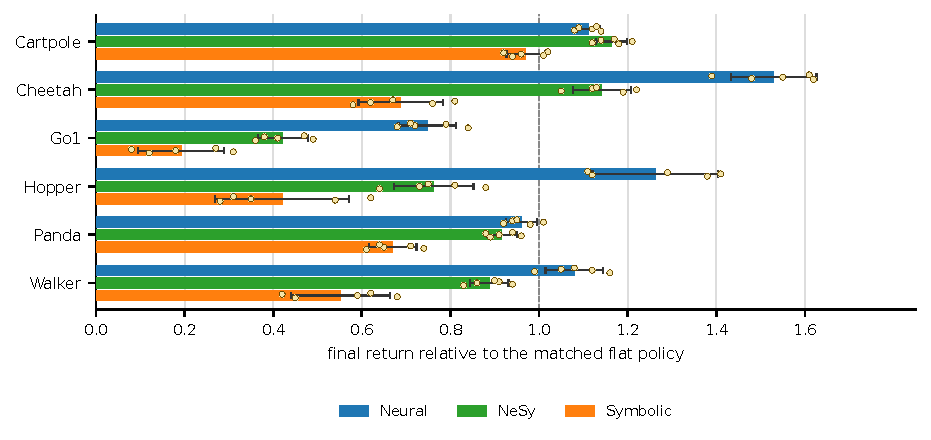
\includegraphics[width=0.93\textwidth]{fig1_sweep.pdf}
\caption{State-based sweep, shown as final return relative to a matched Flat policy. Values above one favor the hierarchical variant. The mixed pattern motivates environment-specific analysis rather than a single global performance claim.}
\label{fig:sweep}
\end{figure*}

\begin{figure*}[!t]
\centering
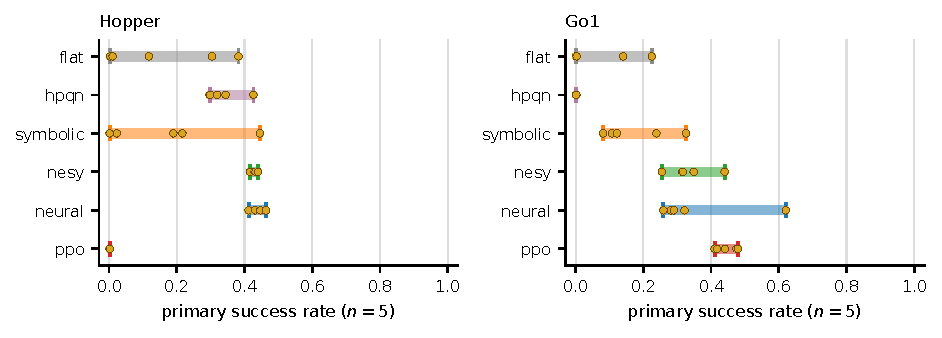
\includegraphics[width=0.99\textwidth]{fig_core_sealed.pdf}
\caption{Matched-budget primary success on Go1JoystickFlatTerrain and HopperHop. Points are seeds. Neural and NeSy finish above Flat on both tasks; HPQN behaves differently across tasks, and PPO reverses its relative position between Go1 and Hopper.}
\label{fig:core}
\end{figure*}

\section{Results}
\subsection{Performance and Robustness}
This subsection addresses Q1 using the state-based sweep, matched-budget Hopper and Go1 comparisons, learning curves, budget sensitivity, action-noise tests, and command/terrain shifts.

\subsubsection{Overview across environments}
Figure~\ref{fig:sweep} reports final environment return relative to Flat. Neural improves Cheetah and Hopper and gives smaller gains on Cartpole and Walker, but falls below Flat on Go1. NeSy improves Cartpole and Cheetah but remains below Flat on the other tasks shown. Symbolic is generally weaker, while Panda is near or below Flat for all three variants. The results therefore depend on both the task and the selection method.

\subsubsection{Matched-budget comparison}
Figure~\ref{fig:core} compares task success after training. On both focal tasks, every Neural seed and every NeSy seed finishes above every Flat seed. The interpretation differs across environments. On HopperHop, HPQN also learns a substantial part of the task, indicating that several behavioral modes are already useful even when their rewards are not specialized. On Go1JoystickFlatTerrain, HPQN collapses near the Flat failure regime, while Neural and NeSy remain substantially higher. The Go1 result therefore depends on skill-specific objectives rather than merely on having several actor heads.

The PPO comparison prevents an over-general conclusion. PPO is weak on Hopper under this matched setup, while it achieves higher average success on Go1; the best Neural run nevertheless exceeds the PPO runs shown. Neural and NeSy can therefore improve the matched Flat implementation without being universally preferable to a strong task-specific optimizer.

\subsubsection{Learning dynamics}
Figure~\ref{fig:allcurves} shows training return across all six environments. On Hopper, Neural and NeSy separate from Flat as training progresses; on other tasks, the methods differ in learning speed, final return, and variability. PPO learns successfully on Cheetah, so its weak Hopper result is not a general failure of the baseline. These curves complement the task-success comparisons by showing how learning develops.

\begin{figure*}[!t]
\centering
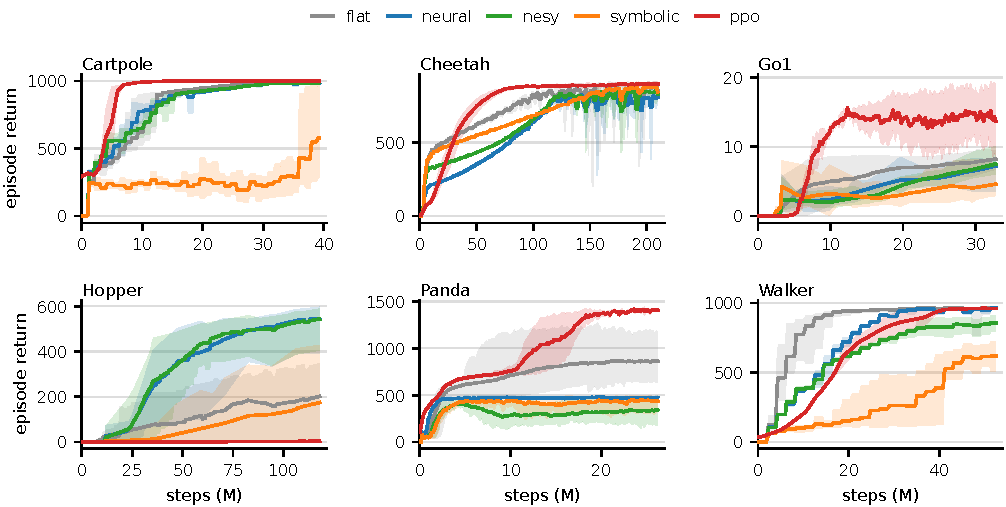
\includegraphics[width=0.95\textwidth]{fig_all_curves_paper.pdf}
\caption{Training return versus environment interaction steps for all six state-based environments. The curves show learning speed, later separation, and variability that post-training summaries omit. Training durations are shown on the horizontal axes; return and task success measure different aspects of performance.}
\label{fig:allcurves}
\end{figure*}

\subsubsection{Budget sensitivity}
The Hopper budget ladder tests whether longer training is enough for Flat to match the hierarchical policies (Fig.~\ref{fig:ladder}). Flat improves initially but gains little at the largest budgets. Neural reaches high success earlier along the ladder, while NeSy reaches a similar level with more training. Some Flat runs overlap the hierarchical results, but increasing Flat's budget does not consistently close the performance difference.

\begin{figure}[!t]
\centering
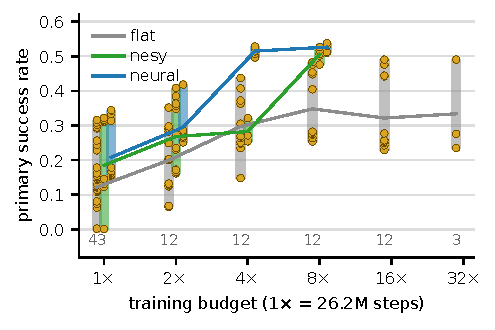
\includegraphics[width=0.98\columnwidth]{fig_ladder.pdf}
\caption{Hopper task success across increasing training budgets. Flat improves initially but gains little at the largest budgets. Neural reaches high success earlier along the ladder, and NeSy reaches a similar level with more training; some individual Flat runs overlap these results.}
\label{fig:ladder}
\end{figure}

\subsubsection{Action-noise robustness}
During evaluation, we add Gaussian noise to the chosen action to test whether policies remain successful when control becomes less precise. The middle and right panels of Fig.~\ref{fig:noise} show the Go1 and Hopper results. Neural and NeSy remain above Flat throughout the tested noise range, although their success generally decreases. Their similar responses do not establish an additional noise-robustness benefit from the symbolic mask. The left panel reports rough-terrain Go1 performance, where PPO performs best.

\begin{figure*}[!t]
\centering
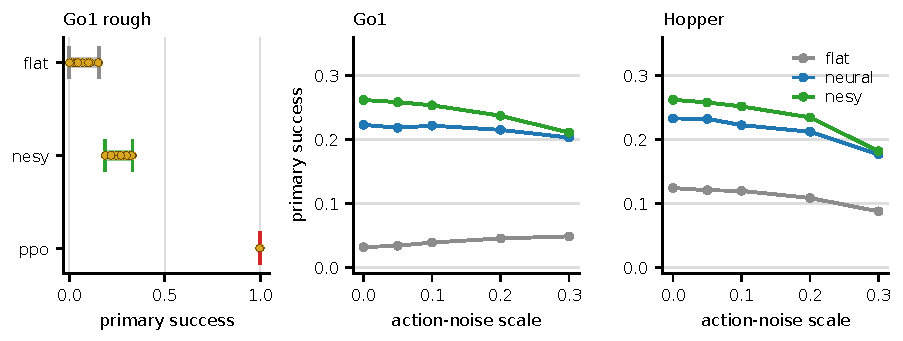
\includegraphics[width=0.98\textwidth]{fig3_reliability.pdf}
\caption{Reliability comparisons. Left: primary success for rough-terrain Go1 evaluation. Middle and right: primary success under increasing evaluation-time action noise on Go1 and Hopper. Neural and NeSy remain above Flat over the tested noise range. Absolute success is shown rather than change normalized to each method's baseline.}
\label{fig:noise}
\end{figure*}

\subsubsection{Go1 command and terrain shifts}
Figure~\ref{fig:go1shift} evaluates rough-terrain Go1 policies under changed conditions without retraining. A command is the desired planar velocity $(c_x,c_y)$ together with desired yaw rate $c_\psi$. ``Stop'' sets the motion command to zero, 1.5 and 2.0~m/s increase the forward command, and the condition labeled ``flat'' evaluates the same rough-trained controller on flat terrain.

The stop condition removes the motion command, so standing safely can satisfy the tracking objective. Higher forward commands reduce success, while rough-to-flat transfer retains some task performance. NeSy generally improves the lowest observed success relative to Flat, whereas Neural shows a wider spread. These results support a task-specific reliability benefit, not a guarantee of successful tracking under every shift.

\begin{figure}[!t]
\centering
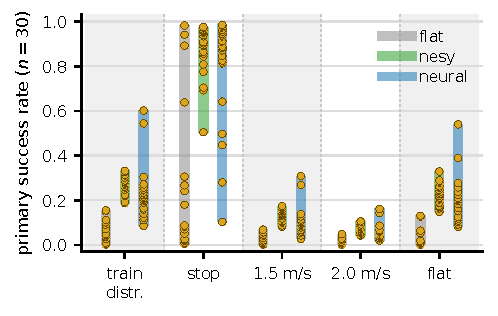
\includegraphics[width=0.98\columnwidth]{fig_oos.pdf}
\caption{Go1 command and terrain shifts for rough-trained policies. ``train distr.'' is evaluation on the training distribution; ``stop'' sets the command to zero; 1.5 and 2.0~m/s increase the forward command; ``flat'' denotes rough-to-flat transfer without retraining.}
\label{fig:go1shift}
\end{figure}

\par\noindent\emph{\textbf{Q1 conclusion.}}
Neural and NeSy outperform Flat in the Hopper and Go1 task-success comparisons and remain stronger under action noise. On Go1, the weak HPQN result supports the importance of skill-specific objectives. NeSy improves lower-end performance under the tested shifts, but PPO achieves higher average Go1 success and is much weaker on Hopper. Hierarchy therefore helps under the tested conditions without providing a universal performance advantage.

\subsection{Skill Behavior}
This subsection addresses Q2 using skill-reward curves, forced execution, and skill removal.

\subsubsection{Skill-reward learning}
Figure~\ref{fig:skillreturns} tracks each hand-written skill reward during NeSy training across all six tasks. The forward-motion rewards grow on Cheetah and Walker, while Cartpole's recovery reward has a large negative early transient. Each curve sums that reward over the whole episode, including steps when another skill acts. It therefore tracks the corresponding objective, not how much that actor contributes to task return. Reward magnitudes also differ by design, so behavioral and removal tests are needed to establish what the skills do.

\begin{figure*}[!t]
\centering
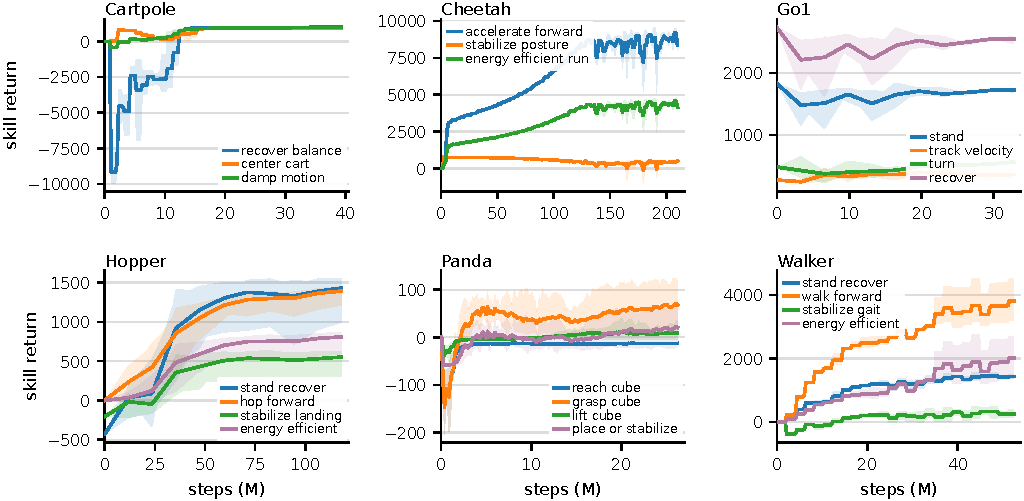
\includegraphics[width=0.95\textwidth]{fig_skill_returns.pdf}
\caption{Per-skill reward accumulated over the episode versus environment interaction steps for hand-written NeSy policies. Each line corresponds to one skill reward and each band is the seed min--max. Rewards include all steps, even when another skill acts, so they do not measure the selected actor's contribution to environment return. Sample sizes are $n=3$ for Cartpole, Cheetah, and Walker, $n=9$ for Panda, and $n=5$ for Go1 and Hopper. Reward scales differ between skills and tasks.}
\label{fig:skillreturns}
\end{figure*}


\subsubsection{Behavioral meaning}
We freeze trained NeSy policies and force each skill to act for a diagnostic rollout. Seven of eight tested Go1 and Hopper skills move the state quantity associated with their semantic objective in the intended direction (probe labels in Fig.~\ref{fig:removal}). The main exception is Hopper's \texttt{energy\_efficient} skill, whose forced behavior is not cleanly distinguished from the other hopping modes. Forced execution therefore tests semantic behavior independently of how often the selector normally uses a skill.

\subsubsection{Skill removal}
We next remove one actor from a trained NeSy policy and let the selector reroute through the remaining skills. Most removals preserve substantial success (Fig.~\ref{fig:removal}), including removal of Go1 \texttt{recover} in many runs. The skill library is therefore behaviorally legible but partly redundant: forced execution tests the intended behavior, while removal tests how much the trained policy depends on that actor.

\begin{figure}[!t]
\centering
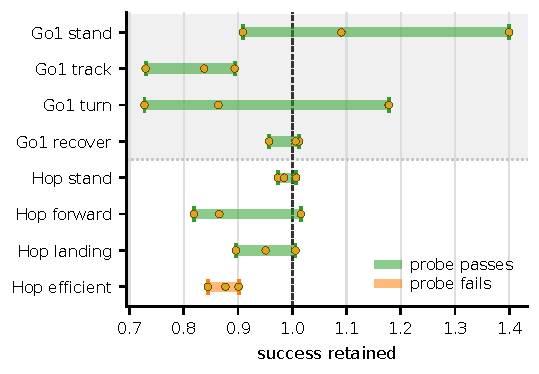
\includegraphics[width=0.96\columnwidth]{fig5_removal_only.pdf}
\caption{Single-skill removal from trained NeSy policies, shown as success relative to each native policy. Values near one indicate retained performance; values above one indicate improvement after removal. Colors mark whether the corresponding forced-skill behavior probe passes or fails. Many removals retain substantial success.}
\label{fig:removal}
\end{figure}

\par\noindent\emph{\textbf{Q2 conclusion.}}
The tested NeSy actors are mostly behaviorally consistent with their semantic names, but the skill library is partly redundant: removing one actor often preserves substantial task success because the learned selector reroutes through other skills. The hierarchy is therefore best described as an interpretable set of behavioral modes rather than a collection of strictly independent causal modules.

\subsection{Symbolic Selection}
This subsection addresses Q3.
\subsubsection{Selector interventions with fixed actors}
We keep trained NeSy actors fixed and change only how skills are chosen. In Fig.~\ref{fig:selector}, \emph{as trained} retains NeSy, \emph{mask removed} allows the learned selector to choose any skill, and \emph{symbolic only} replaces it with the hand-written rule.

On Hopper, removing the mask changes little, whereas replacing learned selection with the fixed rule reduces success. On Go1, removing the mask lowers the weakest results, while fixed selection does not match the best NeSy result. These interventions distinguish restricting the available skills from deciding which available skill should act.

\begin{figure}[!t]
\centering
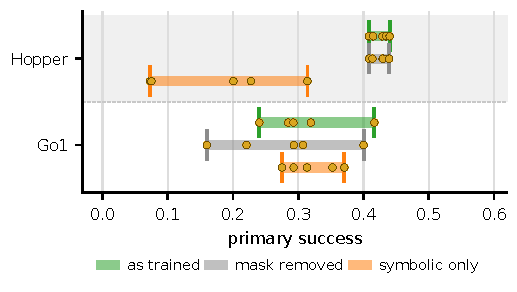
\includegraphics[width=0.98\columnwidth]{fig_selector.pdf}
\caption{Selector interventions with trained NeSy actors held fixed. ``as trained'' retains the original selector; ``mask removed'' disables symbolic filtering; ``symbolic only'' replaces learned selection with the fixed rule. Removing the mask has little effect on Hopper but lowers the weakest Go1 results.}
\label{fig:selector}
\end{figure}

\subsubsection{Fixed symbolic selection}
The Symbolic baseline uses hand-written rules to choose the active skill during both training and evaluation. In Fig.~\ref{fig:core}, it is less consistent on Hopper and generally weaker on Go1 than Neural and NeSy. Together with Fig.~\ref{fig:selector}, this favors learning which skill to use rather than assigning every choice to a fixed rule.

\par\noindent\emph{\textbf{Q3 conclusion.}}
Learning which skill to use is more reliable than relying entirely on the fixed rule. The mask changes little on Hopper but improves the weakest Go1 outcomes. Here, symbolic rules are more useful for restricting choices than for making every decision.

\subsection{Language-Generated Skill Specifications}
This subsection addresses Q4.

\subsubsection{Generation and feedback refinement}
The language extension keeps the reinforcement-learning trainer fixed and replaces the hand-written skill specification. The generator receives a task description, the available semantic state fields, a requested skill count, and a bounded vocabulary of executable reward terms and activation rules. Its output is parsed into skill names, activation conditions, and weighted reward terms; arbitrary generated code is never executed. A validator checks the fields, operators, reward terms, skill count, and always-valid fallback before training.

Feedback refinement returns evaluation statistics to the language model and trains the revised specification from scratch. We compare initial proposals, feedback revisions, and independently resampled proposals; Table~\ref{tab:refineoutcome} also records reward and skill count across refinement iterations. For example, one Cheetah proposal selected \texttt{sprint} on 98.6\% of steps. After feedback, the model increased its forward-velocity weight from 5 to 8, changed the \texttt{stabilize} trigger from $|\text{torso pitch}|>0.5$ to $>0.2$, and lowered the \texttt{smooth\_motion} trigger from joint speed $>10$ to $>6$. These revisions change the skill specification rather than continue training the same policy.

\subsubsection{Results across tasks}
Figure~\ref{fig:llmbars} compares hand-written, initial generated, and feedback-refined specifications across five environments. Cheetah remains close to the hand-written reference in both reward and success. Cartpole and Walker initially lose substantial success despite nonzero shaped reward; refinement improves their results but does not restore the reference performance. Hopper remains near failure, and Go1 success stays low. Table~\ref{tab:llmmain} gives the numerical comparison, while Table~\ref{tab:refineoutcome} records the reward and skill-count changes during refinement.

\begin{figure*}[!t]
\centering
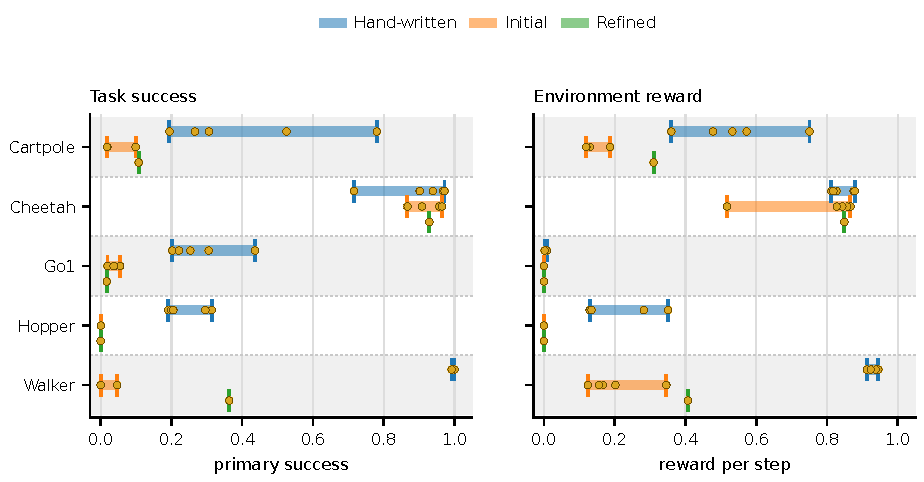
\includegraphics[width=0.90\textwidth]{fig_llm_bars.pdf}
\caption{Language comparison across five environments. Left: deterministic primary success. Right: environment reward per step. Cheetah remains close to the hand-written reference. Initial generated Walker skills receive nonzero reward but almost no task success; the refined run improves success while remaining below the reference. Hand-written and initial conditions show repeated runs; refined is a single final feedback run per environment.}
\label{fig:llmbars}
\end{figure*}

Figure~\ref{fig:usagecartpole} in Appendix~\ref{app:llm} shows skill usage on Cartpole and Cheetah. Cartpole's initial generated policy selects one skill throughout the rollout; refinement spreads selection across several skills but does not recover hand-written performance. Usage describes which skills are selected, whereas Fig.~\ref{fig:llmbars} measures how well the resulting policy performs.

Figure~\ref{fig:llm} shows how task success varies across generated specifications on Cheetah and Walker. Cheetah generally stays near the hand-written reference, although resampling includes weaker runs. Walker's initial proposals range from low success to reference-level performance; feedback revision does not consistently resolve this variation, and the resampled proposals perform poorly. Resampling tests dependence on the particular generated decomposition, while refinement tests whether feedback improves the original proposal. Neither is simply additional training of the same policy.

Schema validation occurs before reinforcement learning, so invalid specifications never enter training. One language model configuration failed the bounded schema on every planned generation attempt, while another produced executable specifications under the same interface. Appendix~\ref{app:llm} gives the generation details.

\begin{figure}[!t]
\centering
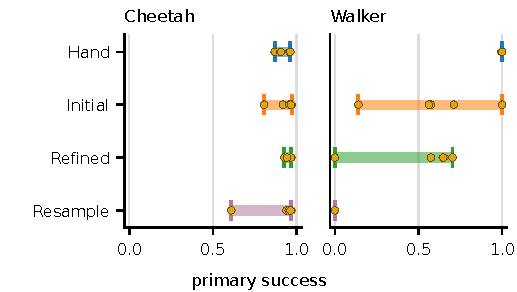
\includegraphics[width=0.98\columnwidth]{fig_controlled_llm.pdf}
\caption{Task success on Cheetah and Walker at a matched RL training budget. Hand-written NeSy is compared with initial, once-refined, and independently resampled specifications. All are trained from scratch. Cheetah is comparatively stable; Walker varies across proposals, and resampling performs poorly.}
\label{fig:llm}
\end{figure}

\par\noindent\emph{\textbf{Q4 conclusion.}}
Language-generated specifications can approach the hand-written reference, most consistently on Cheetah, but executable output does not guarantee a useful decomposition. Walker exposes strong dependence on the generated proposal, and feedback refinement does not reliably recover hand-written performance.


\subsection{Visual Augmentation}
This subsection addresses Q5.

\subsubsection{Scope and visual input}
The comparisons reported here test camera augmentation, not vision-only control. Every condition retains the full privileged state; when enabled, the camera pathway augments only the low-level skill actors. Despite the ``RGB'' label used in code and some figures, the actor input is a $64\times64$ grayscale image stack containing three consecutive frames; the stack supplies temporal information rather than color channels. The image encoder produces features that are concatenated with the same state vector used by the state-only actor. Skill critics, meta-Q, symbolic mask, skill-reward feature extraction, and task-success predicates remain state-based.

The state-only condition uses the same vision-configured environment but disables the actor's camera pathway, keeping the task, reward, and state representation unchanged. The fixed-image condition, labeled \emph{Constant} in figures, keeps the encoder and its extra parameters but feeds the same frozen image at every time step. It therefore tests whether any change comes from informative visual content rather than simply adding a CNN pathway. Representative camera inputs and supplementary rollouts are available on the project website linked at the beginning of the paper.

\subsubsection{Performance and visual information}
Figure~\ref{fig:rgbchange} reports seed-matched changes in evaluation score relative to state-only on Cartpole, Walker, and Cheetah. Walker often improves, but not in every run; Cartpole includes substantial losses, while Cheetah has smaller mixed changes. The pattern does not support a general benefit from adding the camera pathway.

\begin{figure}[!t]
\centering
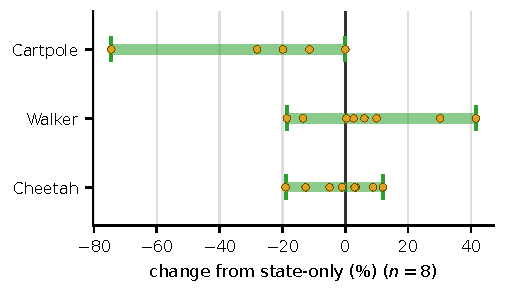
\includegraphics[width=0.96\columnwidth]{fig_rgb_change.pdf}
\caption{Seed-matched percentage change in the reported evaluation score from state-only to state+camera on Cartpole, Walker, and Cheetah. Positive values indicate improvement; negative values indicate a decrease. These relative changes should not be interpreted as a common task-success scale across environments.}
\label{fig:rgbchange}
\end{figure}

\begin{figure*}[!t]
\centering
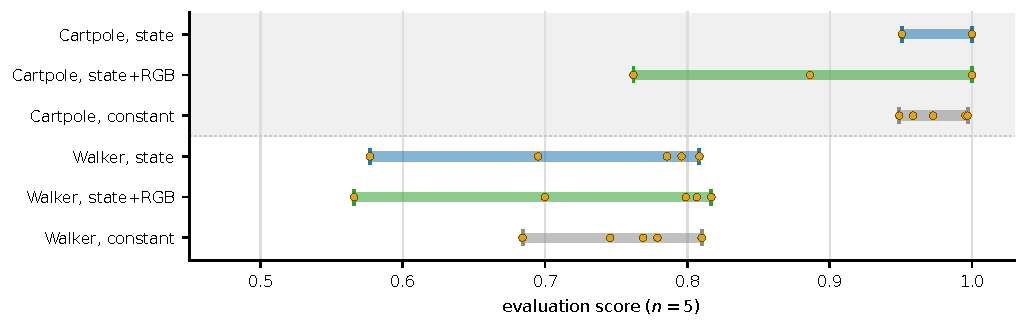
\includegraphics[width=0.96\textwidth]{fig_rgb_controlled.pdf}
\caption{Visual-input evaluation scores on Cartpole and Walker for state-only, state+camera, and fixed-image NeSy. ``state+RGB'' denotes the camera pathway and ``constant'' the fixed-image condition. The overlapping ranges show no clear, consistent camera advantage in this comparison.}
\label{fig:rgbsummary}
\end{figure*}

Figure~\ref{fig:rgbsummary} compares state-only, state+camera, and fixed-image performance on Cartpole and Walker. The overlapping ranges show no consistent camera advantage, although overlap alone does not establish equivalence. The fixed-image condition can perform comparably to live camera input, so the results do not clearly attribute any benefit to informative visual content rather than the added encoder pathway.


\par\noindent\emph{\textbf{Q5 conclusion.}}
Adding the camera pathway does not provide a consistent performance advantage over state-only input. Comparable fixed-image performance also leaves no clear evidence that live visual information improves control under the tested conditions.

\section{Discussion}
\subsection{What the hierarchy contributes}
The results suggest that hierarchy can help organize learning rather than guarantee higher performance. Neural and NeSy improve on Flat AC-PQN, but the HPQN comparison shows that the source of the improvement is task-dependent: multiple actors already help on Hopper, while skill-specific objectives matter on Go1.

\subsection{Behavioral interpretability versus modular necessity}
Here interpretability means that named skills correspond to observable behavioral modes and permit direct interventions. Forced execution tests behavioral meaning, removal tests causal contribution, and selector editing tests symbolic structure. The experiments show meaningful but overlapping skills, so the hierarchy exposes an interpretable control interface rather than a set of strictly independent modules.

\subsection{Reliability and competitiveness are different questions}
A matched Flat ablation tests the effect of the hierarchy, while PPO provides an external performance reference. Neural and NeSy outperform Flat on Hopper and Go1 task success, but PPO achieves higher average success on Go1 and lower success on Hopper. Improving Flat therefore does not establish universal superiority over other RL methods.

\subsection{Language-generated structure}
Language generation is useful only after two checks: the specification must be executable, and independently generated skill sets must produce consistent task behavior. The experiments show that schema validity is necessary but not sufficient, and aggregate training feedback may miss structural errors in reward terms or activation conditions.

\subsection{Visual augmentation}
The camera experiments show why an input pathway needs an information baseline. A policy may become sensitive to images without gaining task performance, particularly when the privileged state already contains the relevant physical variables. The fixed-image condition makes that distinction visible without removing the extra encoder capacity.

\subsection{Limitations}
The study uses manually defined task-success predicates and hand-designed semantic state features. Those choices make the interventions clear but also constrain what the hierarchy can represent. The task set is small relative to the diversity of continuous-control problems, and the strongest performance claims are concentrated on Hopper and Go1. The language pipeline uses a bounded reward/rule vocabulary rather than unrestricted program synthesis. The visual study keeps the high-level selector and critics state-based, so it does not test a fully visual hierarchy. The conclusions apply to the reported training budgets and evaluation settings.

\section{Reproducibility and Contributions}
Code, configurations, analysis utilities, and experiment artifacts are available in the project repository. The results archive records experiment provenance, seed identities, and evaluation products used for the figures and appendix tables.

Rosela Berberi developed and evaluated the visual-input extension and experiments. Anja Koroveshi developed and evaluated the language-generated skill pipeline, including skill generation, feedback refinement and comparison of skill usage across environments. Ivan Smirnov and Maryana Smirnova jointly developed the continuous-control framework and ran the main experiment suite. Ivan focused on algorithm integration, selector and baseline configurations, and experiment orchestration; Maryana focused on environment and reward integration, evaluation tooling, and robustness and skill-intervention analyses. Both contributed to experimental design and result analysis, and all authors contributed to reviewing the final manuscript. Outside the skill-generation experiments, we used LLMs for code development, paper revision and writing. The authors checked this work through personal verification.

\section{Conclusion}
We adapted NEXUS to continuous actions by replacing each discrete low-level policy with a deterministic actor and state--action critic while preserving the discrete semantic selector. Neural and NeSy substantially improve task success and reliability over Flat AC-PQN on Hopper and Go1, but their relation to PPO is task-dependent. The learned skills are mostly behaviorally meaningful but partly redundant, and symbolic rules are most useful as constraints around learned selection rather than as a complete timing policy. Language-generated skills can approach hand-written performance, particularly on Cheetah, but results vary across generated specifications and feedback refinement does not reliably repair weak proposals. Adding a $64\times64$ grayscale three-frame camera pathway to state-aware skill actors does not yield a consistent performance advantage. The main contribution is therefore an experimentally testable account of when semantic structure changes continuous-control learning, which parts of that structure matter, and how generated skills and visual inputs can fail.

\begin{thebibliography}{6}
\bibitem{nexus} Anonymous Authors, ``From Objects to Skills: Interpretable Meta-Policies for Neural Control,'' under review, 2026.
\bibitem{sutton1999} R. S. Sutton, D. Precup, and S. Singh, ``Between MDPs and Semi-MDPs: A Framework for Temporal Abstraction in Reinforcement Learning,'' \emph{Artificial Intelligence}, vol. 112, no. 1--2, pp. 181--211, 1999.
\bibitem{bacon2017} P.-L. Bacon, J. Harb, and D. Precup, ``The Option-Critic Architecture,'' in \emph{Proc. AAAI Conf. Artificial Intelligence}, 2017.
\bibitem{pqn} M. Gallici et al., ``Simplifying Deep Temporal Difference Learning,'' arXiv:2407.04811, 2024.
\bibitem{ppo} J. Schulman, F. Wolski, P. Dhariwal, A. Radford, and O. Klimov, ``Proximal Policy Optimization Algorithms,'' arXiv:1707.06347, 2017.
\bibitem{playground} K. Zakka et al., ``MuJoCo Playground,'' arXiv:2502.08844, 2025.
\end{thebibliography}


\clearpage
\appendices

\section{Language-Generated Skill Protocol}
\label{app:llm}

The language pipeline generates structured skill definitions before RL training. Prompts specify the task, available semantic fields, executable reward terms, activation-rule syntax, and requested skill count. Figure~\ref{fig:llmprompts} shows the Cheetah and Walker examples. The generator configuration reported here is Qwen/Qwen3.8-27B; Qwen2.5-1.5B-Instruct did not produce executable specifications under the schema checks.

\begin{figure*}[!t]
\centering
\setlength{\fboxsep}{8pt}

\fbox{%
\begin{minipage}{0.94\textwidth}
\footnotesize
\textbf{Skill-generation prompt}

\vspace{3pt}

Design a continuous-control NEXUS skillset. Return JSON only:

\texttt{\{"skills": [\{"name":"...", "activation\_rule":"...",}\\
\texttt{\hspace*{1em}"reward\_terms":[\{"type":"...","weight":1.0,"lhs":"..."\}]\}]\}}.

Every scalar field is the same semantic feature supplied to the hand-designed controller.
Fields and units: \texttt{forward\_velocity} in m/s, \texttt{torso\_pitch} in radians,
\texttt{joint\_speed} mean absolute joint angular speed in rad/s, and \texttt{height}
in metres only when listed. No hidden fields or environmental reward are available.

Use EXACTLY the requested skill count and no extra term keys. One skill must have
\texttt{activation\_rule "True"}. Others may overlap. NeSy chooses max learned meta-Q
among allowed skills every step. Define simple complementary goals, not named copies.

Rules: numeric comparisons, \texttt{and/or/not}, \texttt{+ - *}, \texttt{abs(x)},
\texttt{min(x,y)}, \texttt{max(x,y)}. No division.

Rewards sum terms. All weights $>0$ and $\leq10$; penalty types negate their weight internally.

Allowed vocabulary and exact executable semantics:

\texttt{negative\_distance}: \texttt{-weight*abs(lhs-rhs)},
\texttt{-weight*abs(lhs-threshold)}, or \texttt{-weight*abs(lhs)}.

\texttt{positive\_velocity}: \texttt{weight*lhs}.

\texttt{target\_height}: \texttt{weight*clip(lhs/threshold,0,1)};
requires positive \texttt{threshold}, not \texttt{rhs}.

\texttt{binary\_bonus}: \texttt{weight*(lhs>threshold)};
requires \texttt{lhs} and \texttt{threshold}.

\texttt{action\_penalty}: \texttt{-weight*sum(action**2)};
has neither \texttt{lhs}, \texttt{rhs}, nor \texttt{threshold}.

\texttt{posture\_penalty}: \texttt{-weight*abs(lhs)}.

\texttt{rhs} must name another available field, never a number. Constants use
\texttt{threshold} when supported. A terminal penalty of 1 is subtracted from every skill.
Produce between one and six terms per skill.
\end{minipage}
}

\vspace{7pt}

\begin{minipage}[t]{0.455\textwidth}
\fbox{%
\begin{minipage}{0.90\linewidth}
\footnotesize
\textbf{Cheetah task prompt}

\vspace{3pt}

Task: cheetah. Run forward quickly while maintaining posture.

Available fields:
\texttt{forward\_velocity}, \texttt{torso\_pitch}, and \texttt{joint\_speed}.

Skill count: 3.
\end{minipage}
}
\end{minipage}
\hfill
\begin{minipage}[t]{0.455\textwidth}
\fbox{%
\begin{minipage}{0.90\linewidth}
\footnotesize
\textbf{Walker task prompt}

\vspace{3pt}

Task: walker. Walk forward around 1 m/s while remaining upright near 1.2 m torso height.

Available fields:
\texttt{height}, \texttt{torso\_pitch},\\
\texttt{forward\_velocity}, and \texttt{joint\_speed}.

Skill count: 4.
\end{minipage}
}
\end{minipage}

\caption{Language-model prompts used to generate continuous-control skill specifications. The common generation prompt constrains the output to executable reward terms and activation rules; the environment-specific message supplies the task, available semantic fields, and required number of skills.}
\label{fig:llmprompts}
\end{figure*}

A generated proposal is trained without manually modifying its reward terms or activation rules. Evaluation statistics are then returned to the generator for feedback refinement. Figure~\ref{fig:llmfeedback} shows a Cheetah example that requests one revision while keeping the skill count fixed. The generation context and existing proposal are retained during this revision.

\begin{figure*}[!t]
\centering
\setlength{\fboxsep}{8pt}

\fbox{%
\begin{minipage}{0.94\textwidth}
\scriptsize
\textbf{Cheetah feedback-refinement prompt}

\vspace{4pt}

Revise this SAME proposal once using these pilot validation metrics.
Do not add skills. All fields and reward constraints stay the same.

\vspace{5pt}

\texttt{\{}\\
\texttt{\hspace*{1em}"episode\_return\_mean": 463.810302734375,}\\
\texttt{\hspace*{1em}"episode\_return\_std": 59.37163543701172,}\\
\texttt{\hspace*{1em}"episode\_length\_mean": 1000.0,}\\
\texttt{\hspace*{1em}"action\_square\_mean": 0.5742929577827454,}\\
\texttt{\hspace*{1em}"cheetah/action\_norm": 1.8131752014160156,}\\
\texttt{\hspace*{1em}"cheetah/forward\_velocity": 4.647381782531738,}\\
\texttt{\hspace*{1em}"cheetah/forward\_velocity\_mean": 4.647381782531738,}\\
\texttt{\hspace*{1em}"cheetah/joint\_speed": 5.230077743530273,}\\
\texttt{\hspace*{1em}"cheetah/posture\_stable\_rate": 0.9785780906677246,}\\
\texttt{\hspace*{1em}"cheetah/speed\_success\_rate": 0.9164843559265137,}\\
\texttt{\hspace*{1em}"cheetah/torso\_pitch": -0.05432555079460144,}\\
\texttt{\hspace*{1em}"common\_skill\_step/0\_accelerate\_forward": 4.642935752868652,}\\
\texttt{\hspace*{1em}"common\_skill\_step/1\_stabilize\_posture": 0.572869062423706,}\\
\texttt{\hspace*{1em}"common\_skill\_step/2\_energy\_efficient\_run": 2.305461883544922,}\\
\texttt{\hspace*{1em}"primary\_goal\_metric": 4.647381782531738,}\\
\texttt{\hspace*{1em}"primary\_success\_rate": 0.912656307220459,}\\
\texttt{\hspace*{1em}"rules/eligible\_count": 1.035656213760376,}\\
\texttt{\hspace*{1em}"rules/overlap\_fraction": 0.03551562875509262,}\\
\texttt{\hspace*{1em}"skill\_usage/0\_sprint": 0.9855625629425049,}\\
\texttt{\hspace*{1em}"skill\_usage/1\_stabilize": 0.013890624977648258,}\\
\texttt{\hspace*{1em}"skill\_usage/2\_smooth\_motion": 0.0005468750023283064,}\\
\texttt{\hspace*{1em}"common\_skill\_return/0\_accelerate\_forward": 4642.935546875,}\\
\texttt{\hspace*{1em}"common\_skill\_return/1\_stabilize\_posture": 572.8690795898438,}\\
\texttt{\hspace*{1em}"common\_skill\_return/2\_energy\_efficient\_run": 2305.4619140625}\\
\texttt{\}}
\end{minipage}
}

\caption{Example Cheetah feedback prompt. Here, the generator revises an existing proposal once while the task fields, skill count, reward vocabulary, RL trainer, and evaluation procedure remain fixed.}
\label{fig:llmfeedback}
\end{figure*}

The revised specification is trained from scratch under the same RL configuration; only the generated skill specification changes.



\begin{table}[!t]
\caption{Language-generated skill results by environment. Hand-written and initial generated values are mean $\pm$ standard deviation over five seeds; refined values are from one final feedback run per environment. Rewards are environment reward per step, with environment-specific scales.}
\label{tab:llmmain}
\centering
\footnotesize
\setlength{\tabcolsep}{3pt}
\begin{tabular}{@{}lccc@{}}
\toprule
Environment & Hand-written & Initial & Refined\\
\midrule
\multicolumn{4}{c}{Environment reward}\\
\midrule
Cartpole & $0.539\pm0.128$ & $0.135\pm0.026$ & $0.310$\\
Cheetah & $0.842\pm0.029$ & $0.783\pm0.133$ & $0.849$\\
Walker & $0.929\pm0.011$ & $0.199\pm0.078$ & $0.407$\\
Hopper & $0.206\pm0.093$ & $0.000\pm0.000$ & $0.000$\\
Go1 & $0.0064\pm0.0021$ & $\approx0$ & $\approx0$\\
\midrule
\multicolumn{4}{c}{Primary success rate}\\
\midrule
Cartpole & $0.415\pm0.214$ & $0.035\pm0.032$ & $0.108$\\
Cheetah & $0.899\pm0.095$ & $0.913\pm0.042$ & $0.929$\\
Walker & $0.997\pm0.004$ & $0.009\pm0.019$ & $0.363$\\
Hopper & $0.241\pm0.053$ & $0.001\pm0.000$ & $0.000$\\
Go1 & $0.284\pm0.084$ & $0.037\pm0.011$ & $0.017$\\
\bottomrule
\end{tabular}
\end{table}


\begin{table}[!t]
\caption{Separate exploratory feedback-refinement trajectories from iteration 0 to iteration 3, allowing the skill count to change. Each iteration is one training run. These are not the fixed-count, one-revision comparisons in Fig.~\ref{fig:llm}, and iteration 0 is not the multi-seed initial mean in Table~\ref{tab:llmmain}.}
\label{tab:refineoutcome}
\centering
\footnotesize
\setlength{\tabcolsep}{4pt}
\begin{tabular}{@{}lccl@{}}
\toprule
Environment & Reward $0\rightarrow3$ & Skills & Outcome\\
\midrule
Cartpole & $0.140\rightarrow0.310$ & $3\rightarrow5$ & peak at iter.~1\\
Cheetah & $0.743\rightarrow0.849$ & $3\rightarrow5$ & monotonic increase\\
Walker & $0.637\rightarrow0.407$ & $3\rightarrow5$ & net regression\\
Hopper & $0.000\rightarrow0.000$ & $3\rightarrow5$ & no reward signal\\
Go1 & $0.0062\rightarrow0.0000059$ & $3\rightarrow5$ & collapse after iter.~0\\
\bottomrule
\end{tabular}
\end{table}


\begin{figure*}[t]
\centering
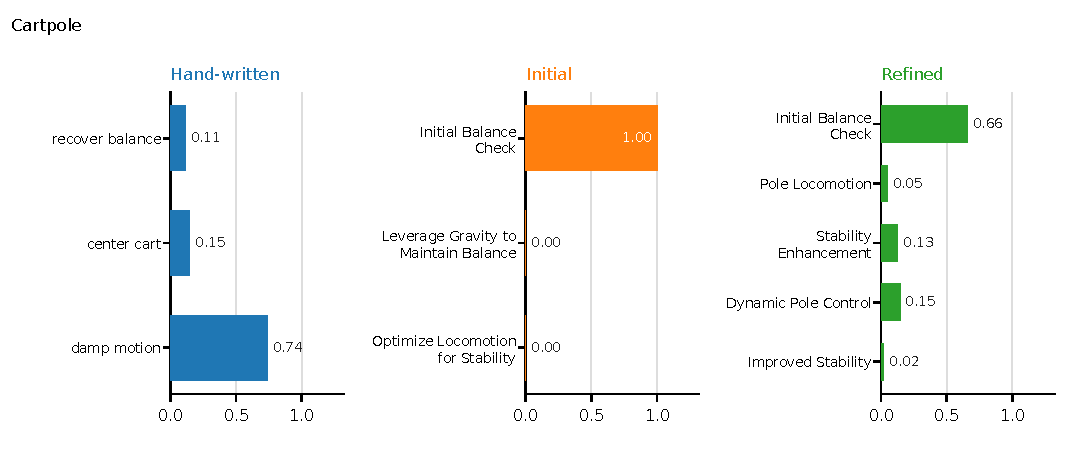
\includegraphics[width=0.98\textwidth]{fig_skill_usage_Cartpole.pdf}\\[3pt]
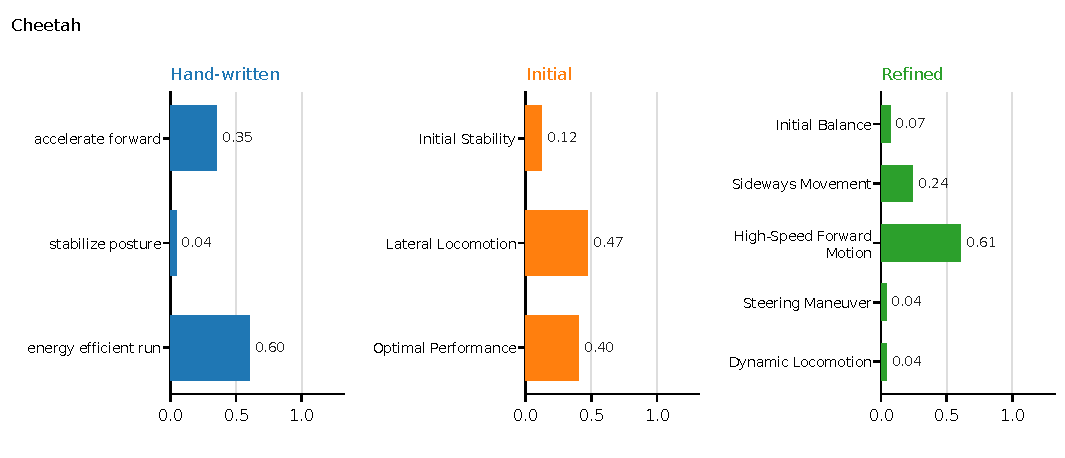
\includegraphics[width=0.98\textwidth]{fig_skill_usage_Cheetah.pdf}
\caption{Skill usage for Cartpole and Cheetah. Each block is the fraction of rollout steps spent in that skill. Generated sets can concentrate selection in a single generic skill; Cartpole's initial set uses one skill on every step.}
\label{fig:usagecartpole}
\end{figure*}




\end{document}